\documentclass[margin,line]{res}

\usepackage{CJKutf8}

\usepackage{graphicx}
\usepackage{float}
\usepackage{tabularx}
\usepackage{hyperref}
\hypersetup{
  colorlinks   = true, %Colours links instead of ugly boxes
  urlcolor     = blue, %Colour for external hyperlinks
  linkcolor    = blue, %Colour of internal links
  citecolor   = red %Colour of citations
}

\oddsidemargin -.5in
\evensidemargin -.5in
\textwidth=6.0in
\itemsep=0in
\parsep=0in
% if using pdflatex:
\setlength{\pdfpagewidth}{\paperwidth}
\setlength{\pdfpageheight}{\paperheight} 

\newenvironment{list1}{
  \begin{list}{\ding{113}}{%
      \setlength{\itemsep}{0in}
      \setlength{\parsep}{0in} \setlength{\parskip}{0in}
      \setlength{\topsep}{0in} \setlength{\partopsep}{0in} 
      \setlength{\leftmargin}{0.17in}}}{\end{list}}
\newenvironment{list2}{
  \begin{list}{$\bullet$}{%
      \setlength{\itemsep}{0in}
      \setlength{\parsep}{0in} \setlength{\parskip}{0in}
      \setlength{\topsep}{0in} \setlength{\partopsep}{0in} 
      \setlength{\leftmargin}{0.2in}}}{\end{list}}


\begin{document}
\begin{CJK*}{UTF8}{gbsn}

\name{苏道毕力格 \vspace*{.1in}}

\begin{resume}



%%%%%%%%%%%%%
%\section{\sc 个人信息}
%\vspace{.05in}
%\begin{tabularx}{\textwidth}{X r}
%博士后研究员 & 1987-09-10日生，蒙古族\\
%\href{http://www.acfr.usyd.edu.au/}{澳大利亚室外机器人中心(ACFR)}, \href{https://sydney.edu.au/}{{悉尼大学}}     &  +61(0)-410-891-777 \\            
%J04 - Rose Street BD, The University of Sydney & daobilige.su@sydney.edu.au \\         
%NSW 2006, Australia   & \\%{\it E-mail:} 
%%博士研究生 & 1987-09-10日生，蒙古族\\
%%自主系统研究中心（CAS）, 悉尼科技大学（UTS）      &  +61(0)-410-891-777 \\            
%%Building 11, Level 9, Room 300         & daobilige.su@gmail.com \\         
%%81 Broadway, Ultimo, NSW 2007, Australia  & \\%{\it E-mail:}  paciorek@stat.cmu.edu\\       
%%  & \\%{\it WWW:} www.stat.cmu.edu/\verb+~+paciorek \\     
%\end{tabularx}

%%%%%%%%%%%%
\section{\sc 个人信息}
\vspace{.05in}
\begin{tabularx}{\textwidth}{X r}
副教授 & 1987-09-10日生，蒙古族\\
\href{http://en.cau.edu.cn/}{中国农业大学 (CAU)}, \href{http://coe.cau.edu.cn/}{工学院}, 机电工程系     &  sudao@cau.edu.cn \\            
北京市海淀区清华东路17号中国农业大学东校区工学院447 & \\         
%NSW 2006, Australia   & \\%{\it E-mail:} 
%博士研究生 & 1987-09-10日生，蒙古族\\
%自主系统研究中心（CAS）, 悉尼科技大学（UTS）      &  +61(0)-410-891-777 \\            
%Building 11, Level 9, Room 300         & daobilige.su@gmail.com \\         
%81 Broadway, Ultimo, NSW 2007, Australia  & \\%{\it E-mail:}  paciorek@stat.cmu.edu\\       
%  & \\%{\it WWW:} www.stat.cmu.edu/\verb+~+paciorek \\     
\end{tabularx}



%%%%%%%%%%%%
\section{\sc 研究方向}
农业机器人, 人工智能, 深度学习, SLAM(同时定位与制图), 机器人导航, 机器人视觉/听觉


%%%%%%%%%%%%
\section{\sc 当前工作}
\begin{tabularx}{\textwidth}{X r}
%\href{http://www.uts.edu.au}{{\bf University of Sydney}}, Sydney, Australia  
副教授, &2020-09 - 至今\\
\end{tabularx}
%{\em Department of Statistics} 
\vspace*{-.1in}
\begin{list1}
\item[] \href{http://en.cau.edu.cn/}{中国农业大学 (CAU)}, \href{http://coe.cau.edu.cn/}{工学院}, 机电工程系, 北京, 中国
\end{list1}
\begin{figure}[H]
  \centering
  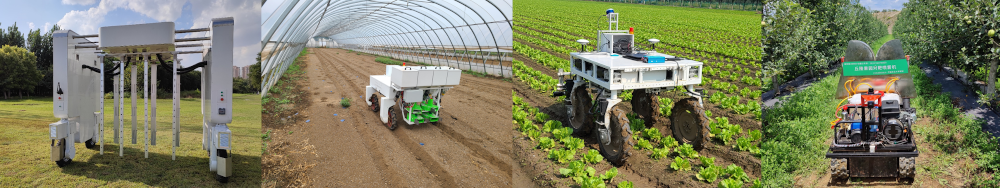
\includegraphics[width=0.99\columnwidth]{./figs/cau_robots_smallsize.png}
  %\caption{The architecture of non-bottleneck-1D block.}
  \label{fig:cau_robots}
\end{figure}

%%%%%%%%%%%%


%%%%%%%%%%%%
\section{\sc 教育背景}
\begin{tabularx}{\textwidth}{X r}
%\href{http://www.uts.edu.au}{{\bf University of Sydney}}, Sydney, Australia  
博士后研究员, &2017-03 - 2020-04\\
\end{tabularx}
%{\em Department of Statistics} 
\vspace*{-.1in}
\begin{list1}
\item[] \href{http://www.acfr.usyd.edu.au/}{澳大利亚室外机器人中心 (ACFR)}, %\\ {\it Expected:} Jan. 2017
\href{https://sydney.edu.au/}{{悉尼大学}}, 悉尼, 澳大利亚
\begin{list2}
\vspace*{.05in}
\item 研究课题:  ``Intelligent Perception Systems for Agriculture and the Environment'' (农业环境的智能感知系统开发)
%\item Dissertation Topic:  ``Hierarchical Models for Multiple Ratings
%  in Performance-Based\\ \hspace*{1.23in} Student Assessments.'' 
\item 导师: \href{http://sydney.edu.au/engineering/people/salah.sukkarieh.php}{Prof. Salah Sukkarieh} (澳大利亚科学院(\href{https://www.atse.org.au/}{ATSE})院士), %\href{http://sydney.edu.au/engineering/people/james.underwood.php}{Dr. James Underwood}
\item \textbf{参与研发的机器人}: \href{https://confluence.acfr.usyd.edu.au/display/AGPub/Our+Robots}{Ladybird, RIPPA, Digital Farmhand, Shrimp} (\href{https://sydney.edu.au/engineering/our-research/robotics-and-intelligent-systems/australian-centre-for-field-robotics/agriculture-and-the-environment.html}{其他链接})
\end{list2}
\end{list1}

\begin{figure}[H]
  \centering
  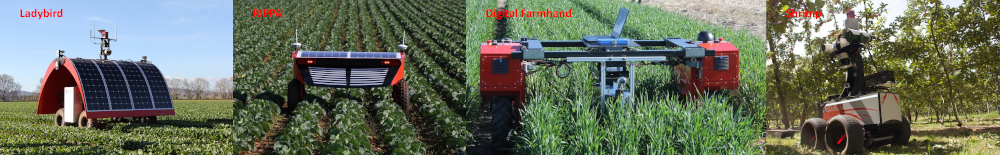
\includegraphics[width=0.99\columnwidth]{./figs/ladybird_rippa_digitalfarmhand_shrimp_smallsize.png}
  %\caption{The architecture of non-bottleneck-1D block.}
  \label{fig:ladybird_rippa_digitalfarmhand_shrimp}
\end{figure}

\begin{tabularx}{\textwidth}{X r}
\href{http://www.uts.edu.au}{{\bf 悉尼科技大学(UTS)}}, 悉尼, 澳大利亚  &2013-03 - 2017-03\\
\end{tabularx}
%{\em Department of Statistics} 
\vspace*{-.1in}
\begin{list1}
\item[] 博士研究生， 机器人领域， \href{http://www.cas.uts.edu.au}{自主系统研究中心（CAS）}%\\ %{\it 预期毕业时间:} 01/2017
\begin{list2}
\vspace*{.05in}
\item 博士课题:  ``Robotic Sound Source Mapping using Microphone Arrays'' 
%\item Dissertation Topic:  ``Hierarchical Models for Multiple Ratings
%  in Performance-Based\\ \hspace*{1.23in} Student Assessments.'' 
\item 导师: \href{http://www.uts.edu.au/staff/jaime.vallsmiro}{A/Prof. Jaime Valls Miro}
\item 副导师:  \href{http://www.uts.edu.au/staff/teresa.vidalcalleja}{Dr. Teresa Vidal Calleja}
\end{list2}
\end{list1}

\begin{tabularx}{\textwidth}{X r}
\href{http://emaro.irccyn.ec-nantes.fr/}{{\bf EMARO} (欧洲先进机器人硕士(EM双学位联合培养项目))} &2010-10 - 2012-10\\
\end{tabularx}
%{\em Department of Mathematics and Statistics} 
\vspace*{-.1in}
\begin{list1}
\item[] 热那亚大学, 意大利 (2011-10 - 2012-10)
\begin{list2}
\vspace*{.05in}
\item 自动化硕士学位, GPA: 92/100
\end{list2}
\begin{list2}
\vspace*{.05in}
\item 硕士课题 完成与 日本庆应大学 (Apr, 2012 - Sep, 2012)\\
硕士课题: Designing Real-Time Robot Audition System (实时机器人听觉系统的设计)\\
导师: Prof. Nozumo Hamada
\end{list2}
\end{list1}
\begin{list1}
\item[] 华沙理工大学, 波兰 (2010-10 - 2011-07)
\begin{list2}
\vspace*{.05in}
\item 自动化与机器人硕士学位, GPA: 81.5/100
\end{list2}
\end{list1}

\begin{tabularx}{\textwidth}{X r}
\href{http://www.zju.edu.cn/english/}{{\bf 浙江大学}}, 中国   &2006-09 - 2010-07\\
\end{tabularx}
%{\em Department of Mathematics and Statistics} 
\vspace*{-.1in}
\begin{list1}
\item[] 机械电子工程学士学位, GPA: 3.63/4.0 (专业课GPA: 3.76/4.0)
\end{list1}



%%%%%%%%%%%%
\section{\sc 代表性项目} 

\begin{itemize}

\item {\bf 无农药除草机器人的智能感知系统开发}\\
2018-09 - 至今, ACFR, 悉尼大学.\\
%Development of a deep learning based method for semantic segmentation of weed against crop using TensorFlow, C++ and ROS. \\
基于深度学习的农作物与杂草的实时语义分割，TensorFlow, C++ and ROS. \\
(企业保密协议项目)\\
\begin{figure}[H]
  \centering
  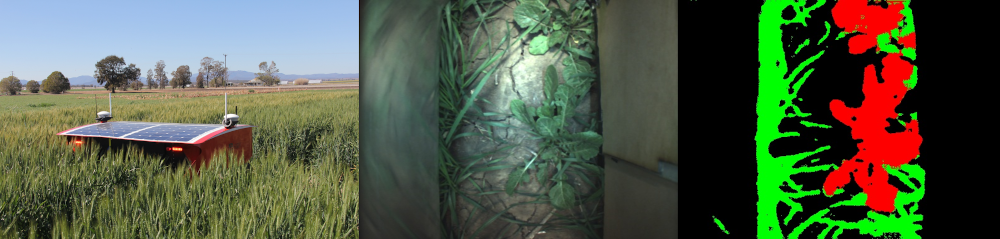
\includegraphics[width=0.9\columnwidth]{./figs/clyde_seg_smallsize.png}
\end{figure}

\item {\bf %Intelligent Perception for Robotic Precision Spray of Vegetable Crops 
蔬菜精确喷洒农药机器人的智能感知系统开发}\\
2017-09 - 2018-09, ACFR, 悉尼大学.\\
%Development of a deep learning based method to detect and track vegetable crops and leaf segmentation and localization for precision spray using TensorFlow.
基于深度学习的蔬菜识别,跟踪, 菜叶分割和定位.用于农业机器人对蔬菜精确喷洒农药.\\
%The method allow an agricultural robot to accurately spray individual leaves of crops. \\
(企业保密协议项目)\\
\begin{figure}[H]
  \centering
  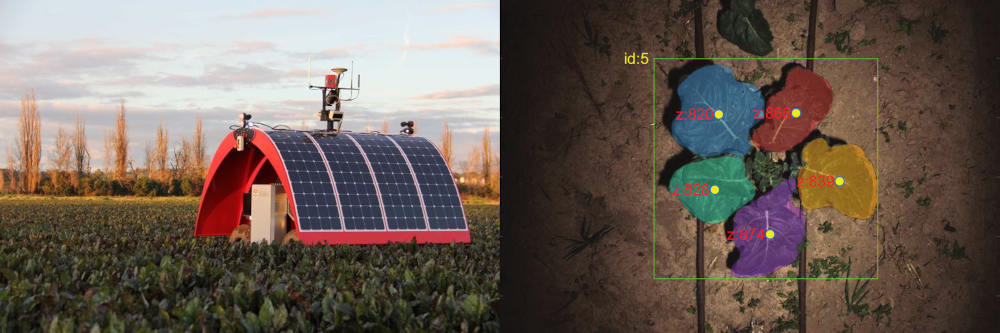
\includegraphics[width=0.62\columnwidth]{./figs/ladybird_leaf_seg_smallsize.png}
\end{figure}


\end{itemize}






%%%%%%%%%%%%
\section{\sc 代表性论文}
%Paciorek, C.J., J.S. Risbey, V. Ventura, and R.D.Rosen. 2002. Multiple indices of Northern Hemisphere Cyclone
%Activity, Winters 1949-1999. Journal of Climate 15:1573-1590.
%
%Paciorek, C.J., R. Condit, S.P. Hubbell, and R.B. Foster.  2000.
%The demographics of resprouting in tree and shrub species of a moist
%tropical forest.  Journal of Ecology 88:765-777.
%
%Paciorek, C.J., B.R. Moyer, R.A. Levin, and S.L. Halpern.  1995.
%Pollen consumption by hummingbird flower mite {\it Proctolaelaps
%  kirmsei} and possible fitness effects on {\it Hamelia patens}.
%Biotropica 27:258-262.  (author order determined by lot)  

\begin{enumerate}
% Su, Daobilige, He Kong, Salah Sukkarieh, and Shoudong Huang. "Necessary and sufficient conditions for observability of SLAM-Based TDOA sensor array calibration and source localization." IEEE Transactions on Robotics 37, no. 5 (2021): 1451-1468.
\item \textbf{Daobilige Su}, He Kong, Salah Sukkarieh and Shoudong Huang, ``Necessary and sufficient conditions for observability of SLAM-Based TDOA sensor array calibration and source localization'', {\it IEEE Transactions on Robotics}, vol. 37 no. 5, pp. 1451-1468, 2021. (2021 \textbf{IF 5.567, 机器人TOP期刊})

%Su, Daobilige, Yongliang Qiao, He Kong, and Salah Sukkarieh. "Real time detection of inter-row ryegrass in wheat farms using deep learning." Biosystems Engineering 204 (2021): 198-211.
\item \textbf{Daobilige Su}, Yongliang Qiao, He Kong and Salah Sukkarieh, ``Real time detection of inter-row ryegrass in wheat farms using deep learning'', {\it Biosystems Engineering}, vol. 204, pp. 198-211, 2021. (2021 \textbf{IF 4.123, 农业综合TOP期刊})

%Su, Daobilige, He Kong, Yongliang Qiao, and Salah Sukkarieh. "Data augmentation for deep learning based semantic segmentation and crop-weed classification in agricultural robotics." Computers and Electronics in Agriculture 190 (2021): 106418.
\item \textbf{Daobilige Su}, He Kong, Yongliang Qiao, and Salah Sukkarieh, ``Data augmentation for deep learning based semantic segmentation and crop-weed classification in agricultural robotics'', {\it Computers and Electronics in Agriculture}, vol. 190, pp. 106418, 2021. (2021 \textbf{IF 5.565, 农业综合TOP期刊})

%Su, Daobilige, Teresa Vidal-Calleja, and Jaime Valls Miro. "Asynchronous microphone arrays calibration and sound source tracking." Autonomous Robots 44, no. 2 (2020): 183-204.
\item {\bf Daobilige Su}, Teresa Vidal Calleja and Jaime Valls Miro, ``Asynchronous microphone arrays calibration and sound source tracking'', {\it Autonomous Robots}, vol. 44 no. 2, pp. 183-204, 2020. (2020 \textbf{IF 3.000})

%Xue, Tengfei, Yongliang Qiao, He Kong, Daobilige Su, Shirui Pan, Khalid Rafique, and Salah Sukkarieh. "One-shot Learning-based Animal Video Segmentation." IEEE Transactions on Industrial Informatics (2021).
\item Tengfei Xue, Yongliang Qiao, He Kong, \textbf{Daobilige Su}, Shirui Pan, Khalid Rafique and Salah Sukkarieh, ``One-shot Learning-based Animal Video Segmentation'', {\it IEEE Transactions on Industrial Informatics}, vol. 18 no. 6, pp. 3799-3807, 2021. (2021 \textbf{IF 10.215, 自动化TOP期刊})
\end{enumerate}







\end{resume}

\clearpage\end{CJK*}
\end{document}




